% Type of the document
\documentclass{beamer}

% elementary packages:
\usepackage{graphicx}
\usepackage[latin1]{inputenc}
\usepackage[T1]{fontenc}
\usepackage[english]{babel}
\usepackage{listings}
\usepackage{xcolor}
\usepackage{eso-pic}
\usepackage{mathrsfs}
\usepackage{url}
\usepackage{amssymb}
\usepackage{amsmath}
\usepackage{multirow}
\usepackage{hyperref}
\usepackage{booktabs}

% additional packages
\usepackage{bbm}

% packages supplied with ise-beamer:
\usepackage{cooltooltips}
\usepackage{colordef}
\usepackage{beamerdefs}
\usepackage{lvblisting}

% Change the pictures here:
% logobig and logosmall are the internal names for the pictures: do not modify them. 
% Pictures must be supplied as JPEG, PNG or, to be preferred, PDF
\pgfdeclareimage[height=2cm]{logobig}{hulogo}
% Supply the correct logo for your class and change the file name to "logo". The logo will appear in the lower
% right corner:
\pgfdeclareimage[height=0.7cm]{logosmall}{Figures/LOB_Logo}

% Title page outline:
% use this number to modify the scaling of the headline on title page
\renewcommand{\titlescale}{1.0}
% the title page has two columns, the following two values determine the percentage each one should get
\renewcommand{\titlescale}{1.0}
\renewcommand{\leftcol}{0.6}

% Define the title.Don't forget to insert an abbreviation instead 
% of "title for footer". It will appear in the lower left corner:
\title[Random Number Generation]{Random Number Generation}
% Define the authors:
\authora{Ksenia Ovadenko} % a-c


% Define the institute:
\institute{Ladislaus von Bortkiewicz Chair of Statistics \\
Humboldt--Universitaet zu Berlin \\}

% Comment the following command, if you don't want, that the pdf file starts in full screen mode:
\hypersetup{pdfpagemode=FullScreen}

%Start of the document
\begin{document}

% create the title slide, layout controlled in beamerdefs.sty and the foregoing specifications

% The titles of the different sections of you talk, can be included via the \section command. The title will be displayed in the upper left corner. To indicate a new section, repeat the \section command with, of course, another section title
%%%%%%%%%%%%%%%%%%%%%%%%%%%%%%%%%%%%%%%%%%%%%%%%%%%%%%%%%%%%%%%%%%%%%%%%%%%%%%%%%%%%%%%%%%%%%%%%%%%%%%%%%%%%%%%%%%%%%%%%
\section{Introduction}

\frame{
\frametitle{Outline}

\begin{enumerate}
\item Applications of Random Numbers 
\item Simple examples of seemingly random sequences:
\begin{itemize}
    \item Linear Congruential Method
    \item Middle Square Method
    \item Mersenne Twister
\end{itemize}
\item RNG and Pseudo RNG
\item Tests for randomness
\item Example of testing a pseudo random sequence in R
\end{enumerate}
}

%%%%%%%%%%%%%%%%%%%%%%%%%%%%%%%%%%%%%%%%%%%%%%%%%%%%%%%%%%%%%%%%%%%%%%%%%%%%%%%%%%%%%%%%%%%%%%%%%%%%%%%%%%%%%%%%%%%%%%%%
\section{Sources of Random Numbers}
%%%%%%%%%%%%%%%%%%%%%%%%%%%%%%%%%%%%%%%%%%%%%%%%%%%%%%%%%%%%%%%%%%%%%%%%%%%%%%%%%%%%%%%%%%%%%%%%%%%%%%%%%%%%%%%%%%%%%%%%

% Subsections are not visible on the actual slide, but are displayed as bookmarks in the pdf file. Their application facilitates an easy navigation trough large pdf files.
%%%%%%%%%%%%%%%%%%%%%%%%%%%%%%%%%%%%%%%%%%%%%%%%%%%%%%%%%%%%%%%%%%%%%%%%%%%%%%%%%%%%%%%%%%%%%%%%%%%%%%%%%%%%%%%%%%%%%%%%
\subsection{}
%%%%%%%%%%%%%%%%%%%%%%%%%%%%%%%%%%%%%%%%%%%%%%%%%%%%%%%%%%%%%%%%%%%%%%%%%%%%%%%%%%%%%%%%%%%%%%%%%%%%%%%%%%%%%%%%%%%%%%%%
\frame{
\frametitle{What is Random Number Generation?}
\textbf{Intuition:} Random Number Generator is a device that generates a sequence of numbers or symbols that \textit{cannot be predicted better than by random chance}
}
%%%%%%%%%%%%%%%%%%%%%%%%%%%%%%%%%%%%%%%%%%%%%%%%%%%%%%%%%%%%%%%%%%%%%%%%%%%%%%%%%%%%%%%%%%%%%%%%%%%%%%%%%%%%%%%%%%%%%%%%
\frame{
\frametitle{Application of Random Numbers}
Depending on the field of application, criteria for randomness can differ
\begin{itemize}
\item Cryptography: the most "demanding" area
\item Statistical Sampling: lower standarts for randomness
\item Monte--Carlo Methods
\item Gambling 
\item Computer Simulation
\end{itemize}
}


%%%%%%%%%%%%%%%%%%%%%%%%%%%%%%%%%%%%%%%%%%%%%%%%%%%%%%%%%%%%%%%%%%%%%%%%%%%%%%%%%%%%%%%%%%%%%%%%%%%%%%%%%%%%%%%%%%%%%%%%
\section{Methods and Algorithms of PRNG}
\frame{
\frametitle{Simple examples of (seemingly) random sequences}
Random sequences should not follow any recognizable pattern. How these sequences can be produced?\\
\bigskip
\textbf{Linear Congruential Generator}
\smallskip
\begin{align}
X_{n+1}=(aX_n+b) \mod m \notag
\end{align}
where\\
\begin{itemize}
    \item \(\emph{a}\), \(\emph{b}\), and \(\emph{m}\) are large integers
    \item\(X_{n+1}\) is the next member of the sequence
     \item The maximum number of numbers formula can produce is \(\emph{m-1}\)
\end{itemize} 

}
%%%%%%%%%%%%%%%%%%%%%%%%%%%%%%%%%%%%%%%%%%%%%%%%%%%%%%%%%%%%%%%%%%%%%%%%%%%%%%%%%%%%%%%%%%%%%%%%%%%%%%%%%%%%%%%%%%%%%%%%
\frame{
\frametitle{Simple examples of (seemingly) random sequences}
\textbf{Middle Square Method}
\begin{center}
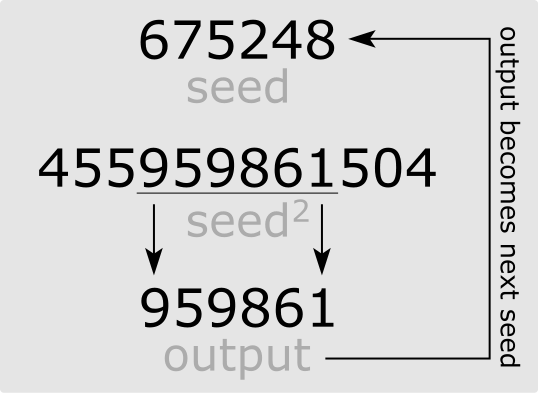
\includegraphics[scale=0.27]{MSM.png}
\end{center}
\begin{itemize}
\item Drawbacks:
    \begin{itemize}
        \item{Short period}
        \item{The output converges to zero} 
    \end{itemize}
\end{itemize}
}

%%%%%%%%%%%%%%%%%%%%%%%%%%%%%%%%%%%%%%%%%%%%%%%%%%%%%%%%%%%%%%%%%%%%%%%%%%%%%%%%%%%%%%%%%%%%%%%%%%%%%%%%%%%%%%%%%%%%%%%%
\frame{
\frametitle{Simple examples of (seemingly) random sequences}
\textbf{Mersenne Twister}
\smallskip
\begin{itemize}
\item Default RNG in Python, R, Ruby, PHP, Stata and some other languages
\item Statistical quality is NOT sufficient for cryptography 
\item Repeat itself after tens thousands of trials
\item Computer's real time clock is used as a seed (milliseconds precision)
\end{itemize}
}

\frame{
\frametitle{Methods and Algorithms of PRNG}
\textbf{Mersenne Twister: Advantages}
\smallskip
\begin{itemize}
\item Relatively fast comparing to other
\item Has a long period which is \( 2^{19937}-1\) (it is not a guarantee of quality) 
\item \(k\)-distributed to 32-bit accuracy for every \( 1\leq k \leq623 \) (uniformly distributed in 623 dimensions)
\item Passes numerous tests for randomness (for example Diehard tests)
\end{itemize}
}


\frame{
\frametitle{Algorithm-Based Random Number Generators}

\begin{itemize}
\item Middle Square Method, Mersenne Twister and Linear Congruential Methods are using algorithms to produce the sequence of seemingly random numbers
\item These sequences are deterministic: they can be predicted, if we know the algorithm and the \emph{seed}
\item A \emph{seed} or a \emph{key} is the first element, from which the computation of the sequence of random numbers starts
\item And they are always periodic (pattern starts to repeat)
\item That is why the number produced are not truly random, but pseudo random
\end{itemize}
}

\frame{


\begin{quote} \textbf{Anyone who considers arithmetic methods of producing random digits is, of course, in a state of a sin.} For [...] there is no such thing as a random number -- there are only methods to produce random numbers, and a strict arithmetic procedure of course is not such a method.\end{quote}
 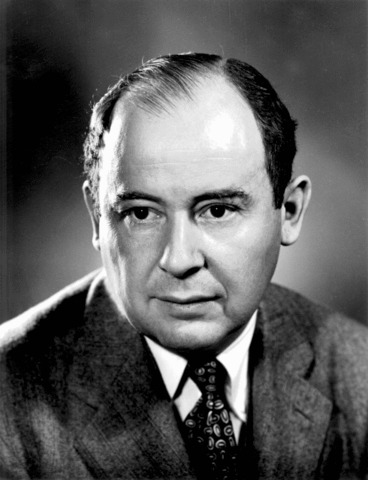
\includegraphics[scale=0.2]{output.jpg}

}

\section{Tests for Randomness}
\frame{
\frametitle{Tests for Randomness}
\begin{itemize}
    \item Statistical properties must be the same as for the sequence of \textbf{i.i.d. uniformly distributed random variables} 
    \item Test for randomness are the test which measure the quality of random numbers.
\end{itemize}
Two examples:
\begin{itemize}
\item Diehards tests: 
    \begin{itemize}
        \item introduced in 1995 by George Marsaglia
        \item contains 12 tests
        \item Mersenne Twister passes all of them
    \end{itemize}
\item Wald--Wolfowitz runs test
\begin{itemize}
\item non-parametric statistical test
\item checks if elements of a two-valued sequence are mutually independent
\end{itemize}
\end{itemize}
}


\section{Random- and Pseudo Random Number Generators}
\frame{
\frametitle{Random- and Pseudo Random Number Generators}
\begin{itemize}
\item To make a sequence truly random, we need a source of entropy
\item The sources of "truly" random numbers are hardware random number generators
\item As the sources of entropy they are having physical processes, either of micro or micro scale
\begin{itemize}
    \item thermal noise
    \item cosmic background radiation
    \item radioactive decay
\end{itemize}
\end{itemize}
}

\frame{
\frametitle{Random- and Pseudo Random Number Generators}
It is possible to use a combined approach:
\begin{enumerate}
    \item Use PRNG algorithm seeded by the source of outer entropy
    \item Make a hybrid which uses the source of naturally occurring entropy when it is available and switches to algorithmic PRNG when the level of entropy drops
\end{enumerate}
}
%%%%%%%%%%%%%%%%%%%%%%%%%%%%%%%%%%%%%%%%
\frame{
\frametitle{For Further Reading}
\begin{thebibliography}{aaaaaaaaaaaaaaaaa}
\beamertemplatearticlebibitems
\bibitem{Oetiker:2006}
Tobias Oetiker, Hubert Partl, Irene Hyna and Elisabeth Schlegl
\newblock{\em The Not So Short Introduction to \LaTeX 2e}
\newblock available on \href{http://www.ctan.org/tex-archive/info/lshort/english/}{www.ctan.org}, 2008
\beamertemplatearticlebibitems
\bibitem{Pakin:2008}
Scott Pakin
\newblock{\em The Comprehensive \LaTeX Symbol List}
\newblock available on \href{http://www.ctan.org/tex-archive/info/symbols/comprehensive/}{www.ctan.org}, 2008
\beamertemplatebookbibitems
\bibitem{Eckel:2004}
Frank Mittelbach and Michel Goossens
\newblock {\em The \LaTeX{ }Companion -- 2nd ed.}
\newblock Addison-Wesley, 2004
\end{thebibliography}
}

%%%%%%%%%%%%%%%%%%%%%%%%%%%%%%%%%%%%%%%%%%%%%%%%%%%%%%%%%%%%%%%%%%%%%%%%%%%%%%%%%%%%%%%%%%%%%%%%%%%%%%%%%%%%%%%%%%%%%%%%
\frame{
\frametitle{For Further Reading}
\begin{thebibliography}{aaaaaaaaaaaaaaaaa}
\beamertemplatearticlebibitems
\bibitem{Trettin:2007}
Mark Trettin and J�rgen Fenn
\newblock{\em An essential guide to \LaTeX 2e usage}
\newblock available on \href{http://tug.ctan.org/cgi-bin/ctanPackageInformation.py?id=l2tabu-english}{www.ctan.org}, 2007
\beamertemplatearticlebibitems
\bibitem{wiki:index}
Wikipedia Wiki Books
\newblock{\em LaTeX-W�rterbuch: InDeX}
\newblock available on \href{http://de.wikibooks.org/}{www.wikipedia.de}
\beamertemplatearticlebibitems
\bibitem{Tantau:2007}
Till Tantau
\newblock{\em User Guide to the Beamer Class, Version 3.07}
\newblock available on \href{http://latex-beamer.sourceforge.net}{www.sourceforge.net}, 2007
\end{thebibliography}
}

% Define the end of the document:
\end{document}
